\documentclass[11pt,numberedappendix,twocolappendix,]{emulateapj}


\usepackage{natbib}
\usepackage{amsmath}
\usepackage{amssymb}
\usepackage{aas_macros}
\usepackage{appendix}
\usepackage{multirow}
\usepackage{color,xcolor}
\usepackage{url}
\usepackage{hyperref}
\hypersetup{colorlinks,linkcolor={blue!50!black},citecolor={blue!50!black},urlcolor={blue!50!black}}

\bibliographystyle{apj}

\renewcommand{\bibname}{References}

\def\water{H$_2$O }
\def\xwater{$x_{\rm H2O,\,1mbar}$ }
\def\preslevel{1.39 mbar\ }
\def\modelE{ROCKE-3D}
\def\CHHHH{CH$_4$}
\def\COO{CO$_2$}
\def\COO{CO$_2$}
\def\memo#1{\color{red}$[${\bf #1}$]$ \color{black}}

\def\Rp{R_{\rm p}}
\def\Rtransit{R_{\rm transit}}
\def\OD#1#2{\frac{d#1}{d#2}}
\def\PD#1#2{\frac{\partial #1}{\partial #2}}

%%%%%%%%%%%%%%%%%%%%%%%%%%%%%%%%%%%%%%%%%%%%%%%%%%%%%%%%%%%%%%%%%%%
\shorttitle{NIR-Driven Moist Upper Atmospheres of Temperate Terrestrial Exoplanets}
\shortauthors{Fujii et al.}

%%%%%%%%%%%%%%%%%%%%%%%%%%%%%%%%%%%%%%%%%%%%%%%%%%%%%%%%%%%%%%%%%%%
\begin{document}

%%%%%%%%%%%%%%%%%%%%%%%%%%%%%%%%%%%%%%%%%%%%%%%%%%%%%%%%%%%%%%%%%%%
\title{NIR-Driven Moist Upper Atmospheres of Synchronously Rotating Temperate Terrestrial Exoplanets}
\author{Yuka Fujii}
\affil{NPP fellow, Universities Space Research Association}
\affil{Goddard Institute for Space Studies, 2880 Broadway, New York, NY}
\affil{Earth-Life Science Institute, Tokyo Institute of Technology, Ookayama, Meguro, Tokyo 152-8550, Japan}
\author{Anthony D. Del Genio}
\author{David S. Amundsen}
\affil{Goddard Institute for Space Studies, 2880 Broadway, New York, NY}
\affil{Department of Applied Physics and Applied Mathematics, Columbia University, New York, NY 10025, USA}

%%%%%%%%%%%%%%%%%%%%%%%%%%%%%%%%%%%%%%%%%%%%%%%%%%%%%%%%%%%%%%%%%%%
\begin{abstract}

\water is a key molecule in characterizing atmospheres of temperate terrestrial planets, and observations of transmission spectra are expected to play a primary role in detecting its signatures in the near future. 
%
Detectability of \water absorption features in transmission spectra primarily depends on the mixing ratio of \water in the upper part of the atmosphere. 
%
While the stratospheric \water mixing ratio of the Earth is as low as $10^{-6}$ due to the cold trap, the efficiency of the cold trap depends on the atmospheric properties. 
%
Here we study the 3-dimensional distributions of \water for synchronously rotating aquaplanets using the general circulation model, {\it ROCKE-3D}, and examine the effect of the  spectra of incident stellar radiation. 
%
We observe a gradual increase of \water mixing ratio in response to the increased incident flux, while the surface temperature around the substellar point is moderate over a wide range of instellation. 
%
At higher incident flux, we find a large-scale circulation in the upper part of the atmosphere, driven by the radiative heating due to the absorption by \water in the upper atmosphere. 
%
The interplay between the efficient vertical transport of \water by this large-scale circulation and the radiative heating appears to play the key role in determining the steady state of the \water mixing ratio in the upper atmosphere.  
%
Consistently, \water mixing ratio is found to be well correlated with the near-infrared portion of the incident flux. 
%
Our results imply that various levels of \water mixing ratios in the upper atmosphere may be expected for synchronously rotating temperate terrestrial planets, and for the more highly irradiated ones the \water absorption features in the transmission spectra are strengthened by factor of a few, loosening the observational demands for a direct H$_2$O detection. 
%
\end{abstract}
%%%%%%%%%%%%%%%%%%%%%%%%%%%%%%%%%%%%%%%%%%%%%%%%%%%%%%%%%%%%%%%%%%%


%%%%%%%%%%%%%%%%%%%%%%%%%%%%%%%%%%%%%%%%%%%%%%%%%%%%%%%%%%%%%%%%%%%
\keywords{exoplanet, atmosphere}

%%%%%%%%%%%%%%%%%%%%%%%%%%%%%%%%%%%%%%%%%%%%%%%%%%%%%%%%%%%%%%%%%%%
\section{Introduction}
\label{s:intro}

One of the primary interests in future observations of Earth-size planets is the presence of \water. 
Knowing what kind of planets harbor it and what do not is an essential ingredient to assess the origin of planetary \water, or to constrain the evolutional pathway. 
It also serves as important prior knowledge to prioritize the targets for identifying biosignatures, on the assumption that \water is a prerequisite for life as we know it. 

\water signatures have been indeed detected in the atmospheres of hot Jupiters \citep[e.g.,][]{Sing2016}. 
However, detecting molecular signatures including \water on temperate terrestrial planets is exceedingly challenging \citep{Cowan2015}, 
because of the small planetary radius and the small scale height (due to the lower temperature and presumably large mean molecular weight), making atmospheric features in transit spectra typically at the order of ppm. 
This requires a significant devotion of telescopes, even in the case where the observational noise is limited by stellar photon noise. 
\water is particularly difficult because, while \water is a dominant opacity source of Earth's atmosphere, the mixing ratio of \water above the troposphere---where the transmission spectroscopy typically probes---is fairly small due to the ``cold trap'', i.e., water vapor evaporated from the surface is transported upward, but it condenses as air rises and cools, and most of it precipitates, leaving the stratosphere fairly dry. 
Several studies of modeling transmission spectra of the Earth found  undesirably weak signatures of \water \citep[e.g.,][]{Ehrenreich2006, Kaltenegger2009, Betremieux2013, Misra2014}. 
However, the efficiency of the cold trap depends on the atmospheric properties in general. 

The mixing ratio in the stratosphere is also closely related to planetary water loss and thus planetary habitability. 
\citet{Kasting1993} considered the maximum stratospheric \water mixing ratio that would allow for a planet to sustain Earth-mass water over the Earth's age, $\sim 3 \times 10^{-3}$, as a criterion for the inner edge of the habitable zone (the threshold for the moist-greenhouse stage). 
Motivated mainly by this ``habitability'' aspect, atmospheric models with different levels of complexity have examined the stratospheric \water with varying planetary properties, or equivalently the efficiency of the cold trap. 

\citet{Kasting1993} and \citet{Kopparapu2013} used a simple 1D model with saturated troposphere and isothermal stratosphere to examine the response of the stratospheric \water mixing ratio to increased instellation. 
They found a transition from an Earth-like dry atmosphere to the water-dominated atmosphere driven by the increase of the surface temperature, when the insolation increases from the solar constant only by 20\%. 
The above-mentioned critical mixing ratio ($\sim 3 \times 10^{-3}$) is reached when the surface temperature is 340 K. 


\citet{Wordsworth2013,Wordsworth2014} argued that the degree of the transport from the surface is represented by $\mathcal{M} = m_v p_v L / m_n p_n c_p T $ where $L$, $c_p$, and $T$ are the specific latent heat of the condensing gas, the specific heat capacity at constant pressure of the non-condensing gas, and surface  temperature, respectively, while $m_{\{v,n\}}$ and $p_{\{v,n\}}$ are molar masses  and the partial pressures of condensing ($v$) or non-condensing ($n$) gases. 
The moist upper atmosphere occurs when $\mathcal{M} > 1$. 
This indicates that the degree of the transport from the surface depends on the atmospheric composition, in particular the abundance of non-condensing gases, in addition to incident flux  \citep{Wordsworth2014}. 
\citet{Wordsworth2013} used 1D radiative-convective models with different levels of CO$_2$ and incident flux, and identified the range of parameters that leads to an inefficient cold trap. 

\citet{Rugheimer2013,Rugheimer2015} combined a 1D radiative-convective model with a photochemical model to assess the effect of the spectral energy distribution of incident stellar spectra on atmospheric profiles, and observed an enhanced water mixing ratio in the stratosphere for planets around late-type stars (while not discussed in detail). 

Inevitably, 1D models rely on several assumptions that cannot be treated within the model, including the global transport of heat and water vapor as well as the effect of clouds. 
Over several years, various 3-dimensional general circulation models (GCMs) revisited the atmospheric structure of terrestrial planets and have demonstrated the importance of taking account of the 3-dimensional circulation and climate heterogeneity \citep[e.g.,][]{Ishiwatari2002,Abe2011,Leconte2013a,Leconte2013b,Wolf2014,Wolf2015}. 
% Abe
%\citet{Abe2011} performed a series of GCM experiments using Atmospheric General Circulation Model 5.4g from the Center for Climate System Research, the University of Tokyo, and pointed out that dry planets with a limited amount of water have stable climate over a wider range of orbital distance than ocean-covered planets. 
% Leconte
%\citet{Leconte2013b}, using the Laboratoire de M\'et\'eorologie Dynamique (LMD) generic climate model, and 
% Wolf
%\citet{Wolf2014, Wolf2015}, using the Community Atmosphere Model version 3 and 4 from the National Center for Atmospheric Research, found that 3-dimensional models are more resistant to increased instellation and have modest surface temperature and low stratospheric water vapor over a wider range of instellation than what 1D models predict. This is primarily due to the unsaturated subsidence region of the Hadley cell, which is not taken into account in 1D models. 
In particular, the 3-dimensional climate may be drastically different from what 1D models suggest for habitable-zone planets around late-type stars, not only due to the difference in the spectral energy distribution of the star but also because they may be synchronously rotating \citep{Dole1964, Kasting1993}, although this need not always occur \citep{Goldreich1966,Leconte2015}.  
%
\citet{Yang2013} pointed out that for tidally-locked planets, the convection around the sub-stellar point produces optically thick clouds which contribute to keep the surface temperature moderate for a much wider range of instellation \citep[see also][]{Yang2014,Way2015,Kopparapu2016}. 
They primarily studied the highest instellation that allows for the model to converge as the proxy for the inner edge. 
While they also presented the stratospheric water vapor, the discussion was limited. 

Motivated by these works on the stabilized climate of planets around late-type stars, we are specifically interested in the water vapor transport  into the upper atmosphere, not only because it affects the water loss rate (and thus conventional criterion for habitable conditions) but also because it limits our ability to detect \water through transmission spectroscopy. 
%
Indeed, the planets around later type stars are best suited for future transit observations for several reasons including the higher transit probability, larger signals in transmission spectra, and the abundance of late-type stars in the nearby universe. 

%The water mixing ratio in the stratosphere of a planet around late-type stars has been controversial and not been fully understood \memo{OK...?}. 
%Some of the 1D atmospheric models \citep{Rugheimer2013, Rugheimer2015} as well as 3D models \citep{Godolt2015} infer orders of magnitude larger water vapor mixing ratio in the stratosphere on planets around late-type stars with similar instellation as the Earth receives, 
%while other 3D GCM models show stratospheric mixing ratio of order of $10^{-6}$ even for planets around M-type stars. 

In order to obtain better insights into the processes that control water vapor mixing ratio in the upper atmospheres of synchronously rotating planets where transit observations probe, we conduct series of experiments with the \modelE \ GCM for planets which receive an amount of energy from the host star similar to the Earth's. 
Using \modelE \ , we calculate the atmospheric dynamic, thermodynamic, and radiative fields up to $0.1$ mbar ($\sim $65 km in the case of the Earth), to be able to sufficiently resolve the stratosphere. 
We specifically study the dependence of water vapor mixing ratio on the incident flux (total incident flux and the spectral type), fixing planetary parameters (radius, gravity, atmospheric composition, and atmospheric pressure). 
We also present mock transmission spectra based on GCM outputs in order to evaluate the detectability of \water signatures with future transmission spectroscopy. 




%%%%%%%%%%%%%%%%%%%%%%%%%%%%%%%%%%%%%%%%%%%%%%%%%%%%%%%%%%%%%%%%%%%
\section{Model}
\label{s:model}

%%%%%%%%%%%%%%%%%%%%%%%%%%%%%%%%%%%%%%%%%%%%
\subsection{GCM experiments}
%%%%%%%%%%%%%%%%%%%%%%%%%%%%%%%%%%%%%%%%%%%%

%%%%%%%%%%%%%%%%%%%%%%%%%%%%%%%%%%%
\begin{figure}[!bh]
    \begin{center}
    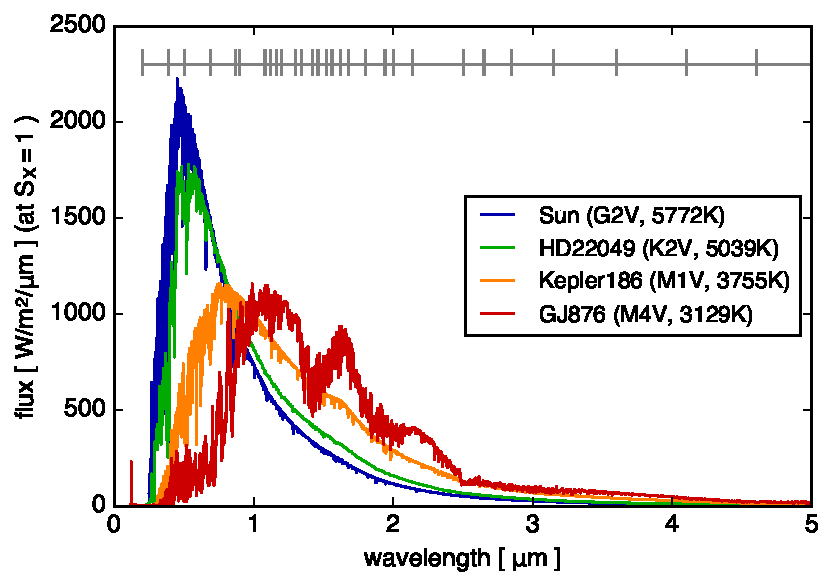
\includegraphics[width=\hsize]{fig/star_spectra.pdf}
    \end{center}
\caption{The spectra of the stars considered in this paper. The flux is normalized so that the total incident flux matches the solar constant. The data sources are \citet{Kurucz1995} (Sun), \citet{Segura2003} (HD 22049), \citet{Allard2012} (Kepler-186), and \citet{Domagal-Goldman2014} (GJ876). The resolution of the spectrum was lowered from the original data just for display purposes. The gray short vertical lines on the horizontal line indicates the short-wave bands used in GCM. }
\label{fig:star_spectra}
\end{figure}
%%%%%%%%%%%%%%%%%%%%%%%%%%%%%%%%%%%



%%%%%%%%%%%%%%%%%%%%%%%%%%%%%%%%%%%
\begin{table*}[btp]
\caption{Stellar Properties}
\begin{center}
\begin{tabular}{ccllllrr} \hline \hline
%
Star & Type & $T_{\rm eff}$ & $L$~[$L_{\odot}$] & $M$~[$M_{\odot}$] & $R$~[$R_{\odot}$] & reference & source of spectrum \\ \hline
%
Sun & G2V & 5772~K & 1 & 1 & 1 & - & \citet{Kurucz1995} \\ 
%
HD 22049 & K2V & 5039~K & 0.32 & 0.82 & 0.74 & \citet{Baines2012} & \citet{Segura2003} \\
%
Kepler 186 & M1V & 3755~K & 0.055 & 0.544 & 0.523 & \citet{Torres2015} & \citet{Allard2012} \\
%
GJ 876 & M4V & 3129~K & 0.0122 & 0.37 & 0.3761 & \citet{vonBraun2014} & \citet{Domagal-Goldman2014} \\ \hline
\end{tabular}
\end{center}
\label{tbl:stellar_properties}
\end{table*}%
%%%%%%%%%%%%%%%%%%%%%%%%%%%%%%%%%%%

We use a GCM named \modelE \ \citep{Way2017} to obtain 3-dimensional atmospheric profiles of planets of our interest. 
\modelE \ is a generalization from the GCM called ModelE2 \citep{Schmidt2014}, which has been developed for the Earth at NASA's Goddard Institute for Space Studies. 
%
The version of the model used here is the same as that used by \citet{Way2016}, and presented in more detail in \citet{Way2017}.
However, the radiation scheme has been replaced by the Suite of Community Radiative Transfer codes based on Edwards and Slingo\footnote{\url{https://code.metoffice.gov.uk/trac/socrates}}~\citep[SOCRATES,][]{EdwardsSlingo1996,Edwards1996} as described in \citet{Way2017}. 
The configuration of the long-wave (thermal) radiation scheme adopted here is as described in \citet{Way2017}, and is the same as that used by the UK Met Office for global atmosphere configuration 7.0 \citep[GA7.0][]{Walters2017}. 
For short-wave (stellar) radiation we use 29 bands, as indicated by the black vertical lines in Figure \ref{fig:star_spectra}, and wavelengths are weighted internally in each band by each stellar spectrum when deriving $k$-coefficients and cloud optical properties to improve accuracy. 
We have SW bands are concentrated in the near-IR regions where H2O absorbs strongly to increase the accuracy of the SW heating


Overlapping gaseous absorption is treated using equivalent extinction~\citep{Edwards1996,Amundsen2016}, and vertical cloud overlap is treated using the mixed maximum-random overlap assumption. 


%The basic architecture of ROCKE-3D is the same as the version used by \citet{Way2016}, but the radiation module has been replaced by the UK Met Office's {\it Socrates} \citep{Edwards1996} after the paper was published. 
%{\it Socrates} utilizes the correlated-k method to compute radiative transfer. 
We used 29 and 9 bands for short wave and long wave, respectively, and the correlated-k method was used to compute radiative transfer. 
We put many bands in the near-IR region where \water absorbs (Figure \ref{fig:star_spectra}) to ensure accuracy of the SW absorption. 
%We paid special attention to the accuracy of the radiative transfer because radiation schemes developed for the Earth system may no longer be accurate when we change the spectral types of the star and/or \water mixing ratio becomes extreme (see the result section below). 
We check the accuracy of the radiation by comparing the radiation calculation in the GCM with higher-resolution calculations, and find a good match;  see Appendix \ref{ap:radiation} for more details. 

The model was configured to have horizontal grids with 4 degree resolution in latitude and 5 degree resolution in longitude, and 40 vertical layers covering up to 0.14 mbar (corresponding to $\sim 65$ km in the case of the Earth). 
Throughout the paper, we consider synchronously rotating planets for their  relevance to the future transmission observations of close-in systems. 

Our atmosphere is 1 bar N$_2$-dominated with 1 ppm CO$_2$, to match the assumption of \citet{Kopparapu2016}. 
We will briefly discuss the dependence on the mixing ratio of CO$_2$ in Section \ref{s:sensitivity}. 
We did not include aerosols. 
Photochemistry is disabled in our model. 

We consider aquaplanets, i.e., planets whose surfaces are wholly covered with water. 
We use a thermodynamic ocean with 50 m depth for the fiducial runs for simplicity. 
However, in Section \ref{ss:sensitivity_ocean}, we also show the results of the runs with fully dynamic ocean, to show that the result is not very sensitive to ocean heat transport. 
The current configuration of the model does not allow us to have an ocean pixel at the south pole. Therefore for convenience we place 1 ``land'' pixel at the south pole. We assume that this tiny fraction of land cover does not have a significant effect on the global climate of the planet, since model fields are minimally asymmetric about the equator. 


%Unlike the majority of the previous GCM works on the terrestrial planets, we calculate the full dynamics of ocean for our fiducial set of runs. 
%We assume 900 meter depth ocean except for the south pole. 
%In Section \ref{ss:sensitivity_ocean}, we also present the results with the q-flux ocean model with zero heat transport, a treatment regularly used in exoplanet GCM community, in order to quantify the sensitivity to the assumption of ocean. 

In our experiments, we mainly changed two parameters: the total incident flux and the spectral type of the star. 
For the latter, four types of stars are considered: 
Sun (G2V), 
HD 22049 (K2V), 
Kepler-186 (M1V), and 
GJ876 (M4V). 
The spectra of HD~22049 and GJ~876 are obtained from \citet{Segura2003} and \citet{Domagal-Goldman2014}, respectively, 
while the spectrum of Kepler-186 is a modeled one using BT-Settl model \citep{Allard2012} based on the stellar parameters reported in Table S1 of \citet{Quintana2014}. 
The physical parameters of these stars as well as the references are summarized in Table \ref{tbl:stellar_properties}, and the spectra are displayed in Figure \ref{fig:star_spectra}. 

The orbital period (= spin period) is changed according to Kepler's 3rd law, to be consistent with the total incident flux the planet receives and the stellar mass. While the incident flux and the orbital period are changed simultaneously for the fiducial set of runs, we also isolate the effect of the orbital period in Section \ref{ss:sensitivity_Porbit}. 

Our fiducial models with thermodynamic ocean typically equilibrate in  $\sim $ 30 Earth years in model time. 
After the steady state is reached, we average the 3-dimensional atmospheric profiles over an integer number of orbits that is approximately 10 Earth years. 
All of the profiles described in the result section are based on the averaged data over 10 Earth years. 


%%%%%%%%%%%%%%%%%%%%%%%%%%%%%%%%%%%
\begin{figure*}[tb]
    \begin{minipage}{0.5\hsize}
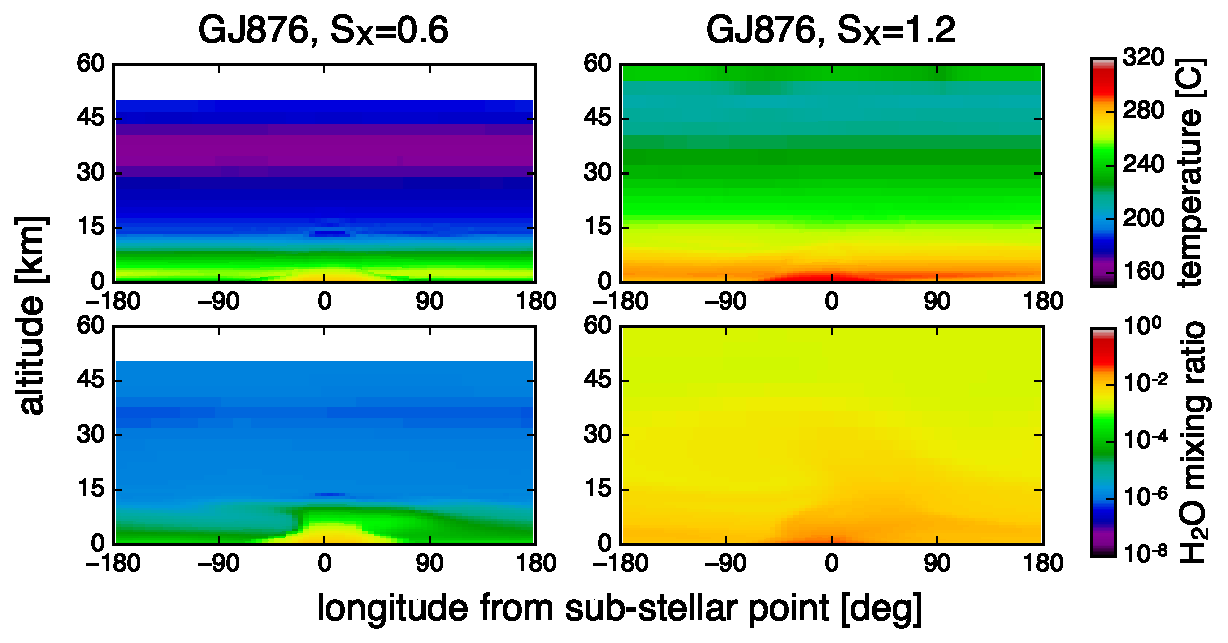
\includegraphics[width=\hsize]{fig/AqOH0TLS_GJ876_temp_xH2O.pdf}
    \end{minipage}
    \begin{minipage}{0.5\hsize}
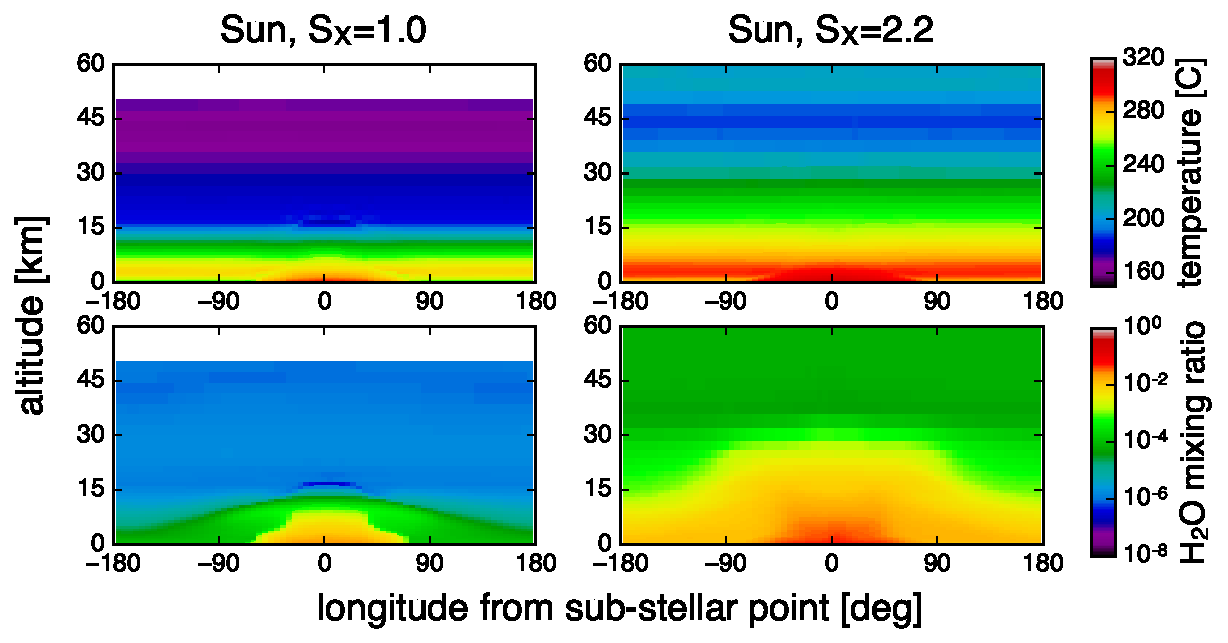
\includegraphics[width=\hsize]{fig/AqOH0TLS_Sun_temp_xH2O.pdf}
    \end{minipage}
    \caption{Profiles of temperature (upper panels) and \water mixing ratio (lower panels) along the equator, for GJ876 (a M4V star; left) and for Sun (right), with different total incident flux ($S_X$). The blank area near the top is above the model top that is  0.14 mbar. }
\label{fig:3Dprofile_equator}
\end{figure*}
%%%%%%%%%%%%%%%%%%%%%%%%%%%%%%%%%%%


%%%%%%%%%%%%%%%%%%%%%%%%%%%%%%%%%%%%%%%%%%%%
\subsection{Simulation of transmission spectra}
\label{ss:method_TransmissionSpectra}
%%%%%%%%%%%%%%%%%%%%%%%%%%%%%%%%%%%%%%%%%%%%

In order to quantify the effect of \water mixing ratio on the absorption features of \water in the transmission spectrum, 
we also simulate it based on the outputs of GCM experiments, setting the model planet in a transiting geometry. 
We follow the procedure described in Appendix B of \citet{Way2017}, which is briefly summarized below. 

First, we obtained the vertical profiles of temperature, water vapor, and cloud particles along the terminator (i.e., dayside-nightside boundary) by linearly interpolating the profiles of the GCM grid points adjacent to the terminator. 
Then, we trace the optical paths of the transmitted ray according to the profile of the refraction index, from the observer toward the stellar disk, in the same way as described in \citet{vanderWerf2008}, following \citet{Misra2014}. 
After that, the spectral opacity at different points along the path is calculated considering Rayleigh scattering and the absorption by atmospheric molecules and cloud particles, but not including the effect of multiple scattering. 
The spectral signatures of the planetary atmosphere are discussed in terms of the transit depth $\Delta F(\lambda )$ where $\lambda $ is the wavelength, as well as the effective height, $h_{\rm eff}$, which is given by
%%%
\begin{equation}
\Delta F(\lambda) = \frac{( R_{\rm p} + h_{\rm eff}(\lambda)  )^2}{R_{\star }^2}. 
\end{equation}
%%%

To compute the absorption coefficient by atmospheric molecules, we use high-resolution line-by-line opacity tables based on HITRAN 2012 database \citep{Rothman2013}, prepared separately from the correlated-k opacity used in the GCM. 
Each line in the HITRAN 2012 database is convolved with the Voigt profile which takes account of Lorentzian pressure broadening and Doppler broadening, 
and the cross sections are computed at varying pressures and temperatures, with a constant interval of the wavenumber grids : $\Delta k = 1\,{\rm cm}^{-1}$. 
The pressure and temperature grids are $P = \{10^{-5},\, 10^{-4},\,...,\,10^3\}$ mbar and $T = \{100,\, 150,\,...,\, 400\}$ K. 
The cross section at a given point along the optical path is obtained by interpolating the values at these lattice points. 

Including the optical effect of clouds is tricky. 
Precisely speaking, one needs to know the size distribution and the spatial distribution of the cloud particles at the time scale of the planetary transit. 
In this paper, we consider the effect of clouds only in an approximate manner with four assumptions. 
%
Firstly, we assume the radius of the cloud particles $r_{\rm cld}$ is $r_{\rm cld}=30~\mu {\rm m}$ (regardless of their phase), similar to the typical values of the ice cloud particles on the Earth as well as in our GCM simulations.  
%
Secondly, the scattering cross section is that of the geometric optics limit, i.e. $2 \pi r_{\rm cld}^2$. 
%
Thirdly, cloud particles are uniformly distributed within each grid cell. 
%
Fourthly, we compute the transmitted light based on the optical properties  averaged over 10 years, rather than computing it based on the instantaneous optical properties and then take the average over years. 
%
The third and fourth points above imply that the effects of clouds we find is the maximum among the possible realization, since loosening these assumptions makes the effective optical thickness due to clouds smaller. 
In that sense, the reality would exist between the cloud-free transmission model and this simplified cloudy transmission model. 
Under these assumptions, the absorption coefficient $\kappa $ is \memo{unnecessary detail?}
%%%
\begin{equation}
\kappa = 2 \pi r_{\rm cld}^2 \cdot n = 3 \rho x_{\rm cld} / ( 2 \rho_{\rm H2O} r_{\rm cld} )
\end{equation}
%%%
where $n$ is the number density of cloud particles, $\rho $ is the density of the ambient atmosphere, $x_{\rm cld}$ is cloud water content, and $\rho_{\rm H2O}$ is the density of liquid/solid water which is assumed to be $1 {\rm g/cm}^3$. 
The uncertainties in the particle radius, scattering cross section, and the cloud water content would change the absorption coefficient by less than a factor of XX \memo{??}.



%%%%%%%%%%%%%%%%%%%%%%%%%%%%%%%%%%%%%%%%%%%%%%%%%%%%%%%%%%%%%%%%%%%
\section{Results}
\label{s:results}
%%%%%%%%%%%%%%%%%%%%%%%%%%%%%%%%%%%%%%%%%%%%%%%%%%%%%%%%%%%%%%%%%%%


%%%%%%%%%%%%%%%%%%%%%%%%%%%%%%%%%%%%%%%%%%%%
\subsection{General Trend in 3D Atmospheric Profiles}
\label{ss:result_H2Omixingratio}
%%%%%%%%%%%%%%%%%%%%%%%%%%%%%%%%%%%%%%%%%%%%


Before examining the dependence of the \water mixing ratio in the upper atmosphere, we shall show the 3-dimensional profiles of temperature and water vapor. 
This is because we need to know at which altitude the mixing ratio of the \water becomes relatively uniform, to identify what kind of \water mixing ratio can be regarded as representative of the humidity in the upper atmosphere. 

Figure \ref{fig:3Dprofile_equator} exhibits the profiles of temperature and \water mixing ratio along the equator for planets around GJ876 (M4V) and around the Sun (G2V), respectively, with varying incident flux. 
In all panels, the substellar point corresponds to the longitude of $0^{\circ }$. 
In general, temperature and \water mixing ratio strongly depend on the distance from the substellar point near the surface, but are fairly uniform in the upper part of the atmosphere. 
Above 1 mbar, which is at 35-50 km altitude depending on the atmospheric temperature profiles, \water mixing ratio becomes horizontally uniform within a few tens of percent. 
The mixing ratio changes by less than an order of magnitude above the 1 mbar level. 
Therefore, in the following, we denote globally averaged \water mixing ratio at \preslevel  by \xwater, and use it as representative of \water abundance in the upper atmosphere. 



We also observe optically thick clouds around the sub-stellar point and the resultant increase of planetary albedo as a function of total incident flux (not shown in figures), consistent with \citet{Yang2013,Yang2014}, \citet{Kopparapu2016} and \citet{Way2016}. 
This indicates the climate-stabilizing effect of clouds, having a negative feedback for the surface temperature, which is pointed out by \citet{Yang2013}. 
As shown in Figure \ref{fig:3Dprofile_equator}, the maximum surface temperature does not exceed 320 K even in highly irradiated cases in our experiments, where \water mixing ratio near the model top is as high as $10^{-3}$; we will discuss this in the subsequent sections. 


%%%%%%%%%%%%%%%%%%%%%%%%%%%%%%%%%%%%%%%%%%%%
\subsection{Response of \water Mixing Ratio to Increased Incident Flux}
\label{ss:result_H2Omixingratio}
%%%%%%%%%%%%%%%%%%%%%%%%%%%%%%%%%%%%%%%%%%%%


%%%%%%%%%%%%%%%%%%%%%%%%%%%%%%%%%%%
\begin{figure*}[!tb]
    \begin{center}
    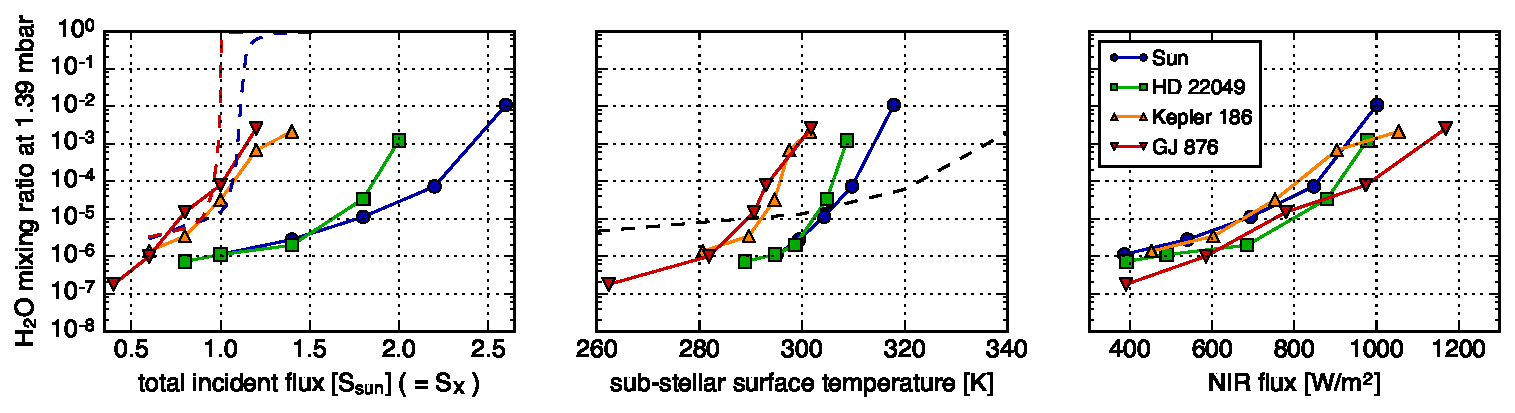
\includegraphics[width=\hsize]{fig/xH2O_3panels.pdf}
    \end{center}
\caption{Water mixing ratio at \preslevel mbar as a function of total incident flux (left), the surface temperature around the sub-stellar point (center), and the near-infrared portion of the incident flux integrated over 0.9-3.0 $\mu $m (right). The colors represent the stellar types: Sun (navy), HD22048 (green), Kepler-186 (orange), and GJ876 (red). Dashed lines are adopted from \citet{Kasting1993}. }                                                                                                             
\label{fig:xH2O_S0X}
\end{figure*}
%%%%%%%%%%%%%%%%%%%%%%%%%%%%%%%%%%%

In this section, we examine in more detail how \water mixing ratio in the upper atmosphere depends on the incident flux (the total flux plus the spectral distribution) when other parameters are fixed. 

The left panel of Figure \ref{fig:xH2O_S0X} presents \xwater versus the total incident flux normalized by the solar constant, indicated by $S_X$ in the following. 
Overall, we find a gradual increase of \xwater as a function $S_X$. 
The slope is much more gradual than suggested by 1D models, in particular those  of \citet{Kasting1993} and \citet{Wordsworth2013} with small CO$_2$ mixing ratio, which typically predict a rapid transition from an Earth-like dry stratosphere to an \water-dominated atmosphere. 
Our result that \water mixing ratio responds more slowly to the incident flux is qualitatively consistent with \citet{Yang2013} who studied synchronously rotating planets around M-type and K-type stars using CAM3 with an emphasis on the stability of the climate. 
Note that we cannot directly compare with their results as the assumptions do not match perfectly; specifically, \cite{Yang2013} assumed a super-Earth with larger radius ($R=2R_{\oplus}$) and higher gravity ($g=1.4g_{\oplus}$), an N$_2$-dominated atmosphere with 400 ppm of CO$_2$, and a 60-day orbital period. 
The dependence on these other planetary parameters will be investigated in the future. 

Because these are synchronously rotating planets which form climate-stabilizing clouds around the sub-stellar point, one might think that the stabilized surface temperature would explain the gradual response of \water to the increased total incident flux. 
To see the effect of the surface temperature, we now plot \xwater as a function of surface temperature around the sub-stellar points where the most convection occurs (Figure \ref{fig:xH2O_S0X}, middle panel). 
It is then clearly seen that the \water mixing ratio starts to rise at a fairly modest surface temperature and increases even more dramatically as a function of surface temperature than 1D models suggest. 
This suggests the increasing surface temperature alone cannot explain the increased stratospheric H2O mixing ratios. 
We will examine this in the next subsection. 

%%%%%%%%%%%%%%%%%%%%%%%%%%%%%%%%%%%%%%%%%%%%
\subsection{Development of Large-Scale Circulation in the Upper Atmosphere}
\label{ss:result_omega}
%%%%%%%%%%%%%%%%%%%%%%%%%%%%%%%%%%%%%%%%%%%%


%%%%%%%%%%%%%%%%%%%%%%%%%%%%%%%%%%%
\begin{figure*}[htb]
    \begin{center}
    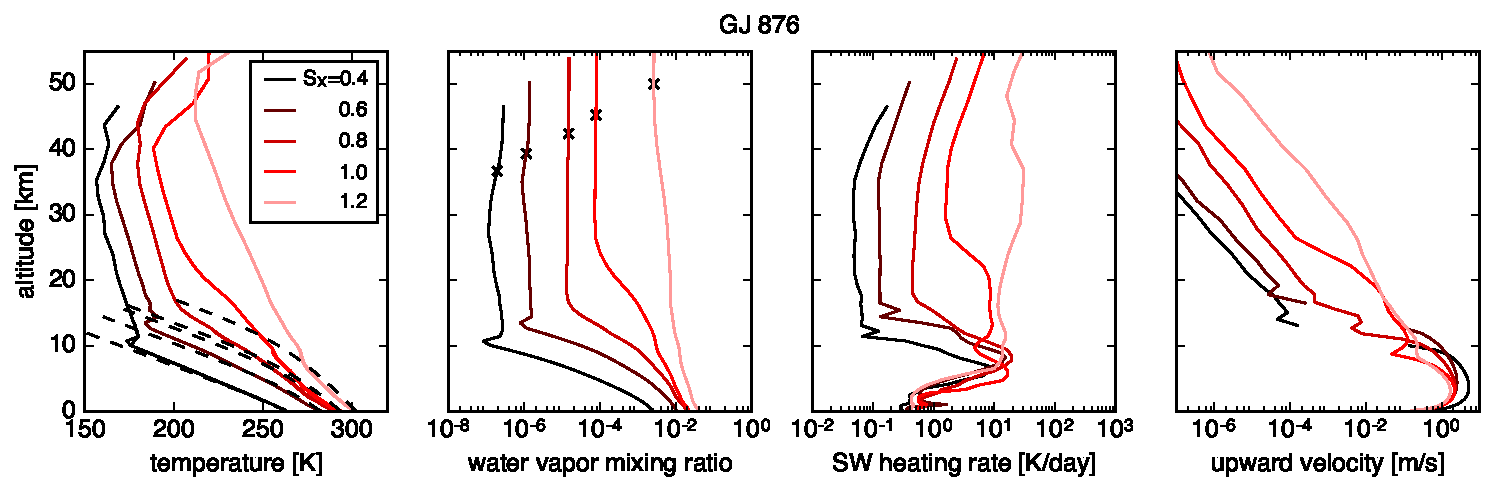
\includegraphics[width=1\hsize]{fig/AqOH0TLS_GJ876_temp_xH2O_vz_heat.pdf}
    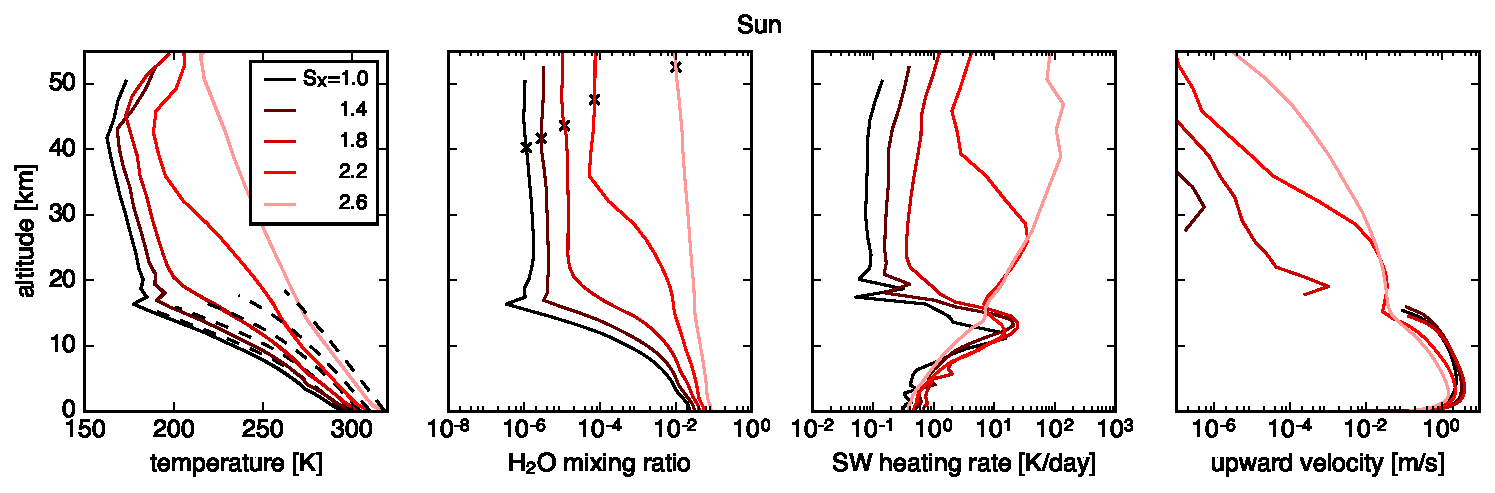
\includegraphics[width=1\hsize]{fig/AqOH0TLS_Sun_temp_xH2O_vz_heat.pdf}
    \end{center}
\caption{From left to right, the vertical profiles of temperature, \water mixing ratio, short-wave heating rate, and upward velocity, averaged of $0.2R_{\oplus }$ of the substellar point, for a planet around GJ876 (top) and around the Sun (bottom) with varying total incident flux. Dashed lines in the left panels show the moist adiabat drawn from the same surface temperature. The cross marks indicate the altitude at \preslevel where  $x_{\rm H2O}$ are measured. }
\label{fig:AqOH0TLS_GJ876_temp_xH2O_vz_heat}
\end{figure*}
%%%%%%%%%%%%%%%%%%%%%%%%%%%%%%%%%%%

In Figure \ref{fig:AqOH0TLS_GJ876_temp_xH2O_vz_heat}, we show the vertical  profiles of temperature, \water mixing ratio, short wave heating rate, and the upward velocity, averaged over the region around the sub-stellar point within the distance of $0.2R_{\oplus }$. 
The dispersion among the different columns is negligible compared to the changes due to varying $S_X$. 
At large incident flux, we observe the development of the vertical motion of the air above the convection layers, concurrently with the increase in \water mixing ratio and the heating rate in the upper atmosphere. 
This large-scale circulation can be naturally explained as follows. 

When the incident flux increases, the heating rate due to the absorption by water vapor also increases. 
The air will then react by rising and adiabatically cooling according to the conservation equation for the potential temperature $\Theta $:
%%%
\begin{equation}
\frac{d\Theta }{dt} + ( {\bf v} \cdot \nabla ) \, \Theta = Q_r + Q_l, \label{eq:conserv_energy}
\end{equation}
%%%
or
%%%
\begin{equation}
\frac{d\Theta }{dt} + u \frac{d\Theta }{dx} + v \frac{d\Theta }{dy} + \omega \frac{d\Theta }{dp} = Q_r + Q_l. \label{eq:conserv_energy_2}
\end{equation}
%%%
where $Q_r$ and $Q_l$ are the radiative and latent heating rates, $\{ u, v, \omega \}$ are the conventional velocity components toward the east ($x-$axis), north ($y-$axis), and upward ($z-$axis; $\omega \equiv  dp/dt$), respectively. 
The latent heating, $Q_l$, is negligible compared to radiative heating above the altitude to which convection penetrates, so it may be dropped. 
Likewise, around the sub-stellar point, the vertical advection may be expected to dominate over the horizontal advection since horizontal gradients are small (Figure \ref{fig:3Dprofile_equator}), thus the second and the third terms in equation (\ref{eq:conserv_energy_2}) may be dropped as an approximation. 
Then, the increase of heating rate, $Q_r$, has the effect of increasing the fourth term in the left-hand side of equation (\ref{eq:conserv_energy_2}). 
Because the upper atmosphere is stable against convection, i.e., $d \Theta / d p < 0 $, larger (positive) $Q_r$ leads to a larger absolute value for $\omega $ (with negative sign), which means the upward motion develops. 

The upward motion of the atmosphere transports water vapor from the moist lower atmosphere to the upper atmosphere, lowering the vertical gradient of water vapor and increasing the moisture at altitude, further increasing the absorption by water. 
This interplay between the radiative heating and water vapor transport eventually finds the steady state where $d\Theta/dt = 0$, leaving the  circulation in the upper atmosphere around the sub-stellar point. 
% This circulation could take over the role of transporting water vapor from the convection that takes place in the lower atmosphere.



%%%%%%%%%%%%%%%%%%%%%%%%%%%%%%%%%%%
\begin{figure*}[htb]
    \begin{center}
    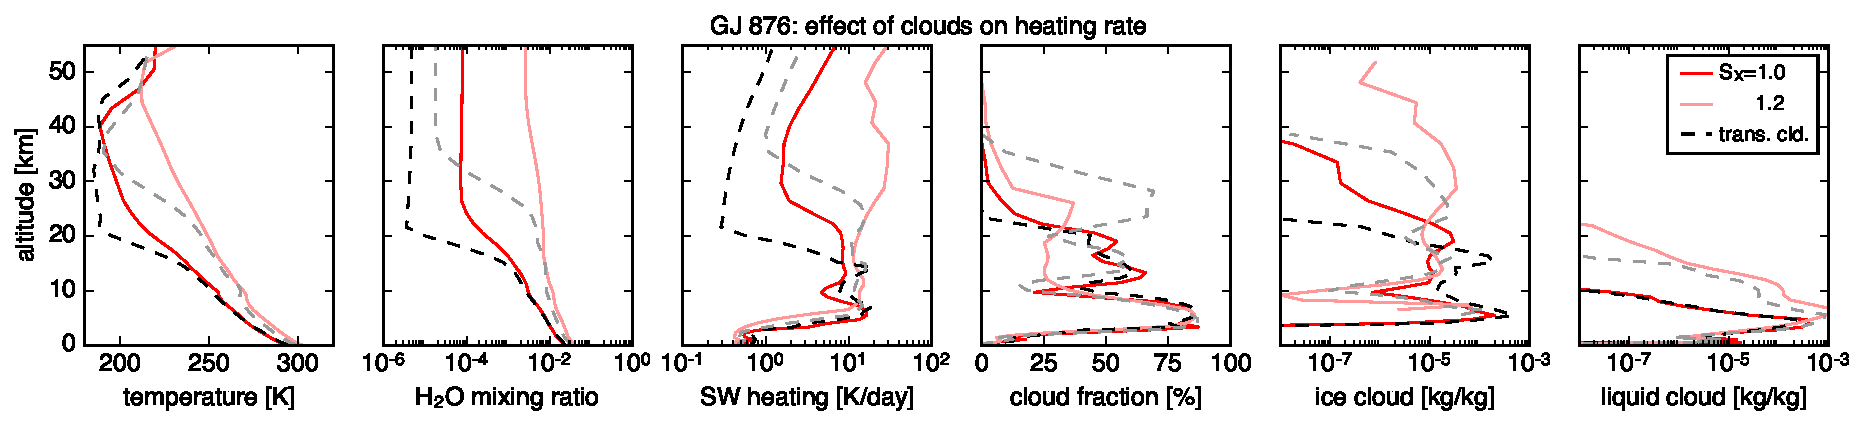
\includegraphics[width=1\hsize]{fig/GJ876_heat_cld.pdf}
    \end{center}
\caption{}
\label{fig:GJ876_heat_cld}
\end{figure*}
%%%%%%%%%%%%%%%%%%%%%%%%%%%%%%%%%%%

This positive feedback between the radiative heating rate and \water mixing ratio in the upper atmosphere would make a modest increase of the radiative flux result in an almost order-of-magnitude increase of water vapor. 
As a result, while the surface temperature increases with $S_X$ only modestly, the upper atmosphere gains moisture more rapidly.  

This picture suggests that the driving factor is the incident flux that reacts with water vapor efficiently, which is the near-infrared part of the incident flux. 
Indeed, as shown in the right panel of Figure \ref{fig:xH2O_S0X}, a good correlation is found between the \water mixing ratio in the upper atmosphere and the near-infrared portion of the incident flux, integrated over 0.9-3 $\mu {\rm m}$ (the interval is somewhat arbitrary), insensitive to the stellar spectral types. 



%%%%%%%%%%%%%%%%%%%%%%%%%%%%%%%%%%%%%%%%%%%%
\subsection{Transmission Spectra}
\label{ss:result_TransmissionSpectra}
%%%%%%%%%%%%%%%%%%%%%%%%%%%%%%%%%%%%%%%%%%%%

In this subsection, we exhibit the transmission spectra for the modeled planets around one of our M-type stars, GJ~876. 
Figure \ref{fig:transmission} shows the transmission spectra in the cases of $S_X=0.6$, $1.0$ and $1.2$, where \water mixing ratio at \preslevel is roughly $10^{-6}$, $10^{-4}$ and $3\cdot 10^{-3}$. 
The vertical profiles at the sub-stellar points are shown in Figure \ref{fig:AqOH0TLS_GJ876_temp_xH2O_vz_heat}, and note that the \water mixing ratio is even higher at medium altitudes (10-30 km). 
Although the refraction due to the planetary atmosphere is included, it causes negligible effects for a temperate planet around late-type stars like GJ 876 \citep{Betremieux2014,Misra2014}. 


Without the opacity due to clouds (dashed lines in Figure \ref{fig:transmission}), the effective altitude of the water vapor absorption features grow from $\sim $10 km to $\sim $40 km when $S_X$ increases from $0.6$ to $1.2$. 
This level of effective altitude of water signatures is comparable with the strongest features in the modeled visible-to-NIR transmission spectrum of the Earth \citep[e.g.,][]{Kaltenegger2009}, thus for the highly-irradiated ones shown here \water signatures can naturally be targeted at as well when trying to observe any of the atmospheric signatures of planets similar to the Earth. 

However, the cloud particles also exist in the upper atmosphere around the terminator, and therefore inclusion of clouds in the way described in Section \ref{ss:method_TransmissionSpectra} substantially raises the bottomline of the transmission spectra. 
%These clouds around the sub-stellar point are presumably transported from around the sub-stellar point, and the cloud water content is at most $\sim 10^{-6}$ [kg/kg] near the cloud top (mostly icy particles) and $\sim 10^{-4}$ [kg/kg] toward the lower atmosphere (liquid particles). 
%
These clouds around the terminator presumably form from water vapor that is transported from the substellar point and cools radiatively or adiabatically. 
%
% But water vapor can be transported from the substellar point to the terminator, and to the extent that it either gently rises and cools adiabatically as it does so, or cools radiatively as it does so, it can saturate and form thin clouds at the terminator.  It has to be one or a combination of those mechanisms that is responsible for forming those clouds.
%
Although these tenuous clouds at high altitude would be optically thin if viewed  from the ground, the grazing geometry of the transmission observation makes it affect the transmission spectra due to the significantly long optical path length. 
We must note, however, that our calculation is likely to overestimate the opacity of clouds as discussed in Section \ref{ss:method_TransmissionSpectra}, because we used an spatially and temporally averaged cloud properties of individual GCM grid cells. 
Thus the reality would exist somewhere between the solid and dashed lines. 
A more realistic modeling of cloud particles will be the scope of future work. 



%%%%%%%%%%%%%%%%%%%%%%%%%%%%%%%%%%%
\begin{figure}[!h]
    \begin{center}
    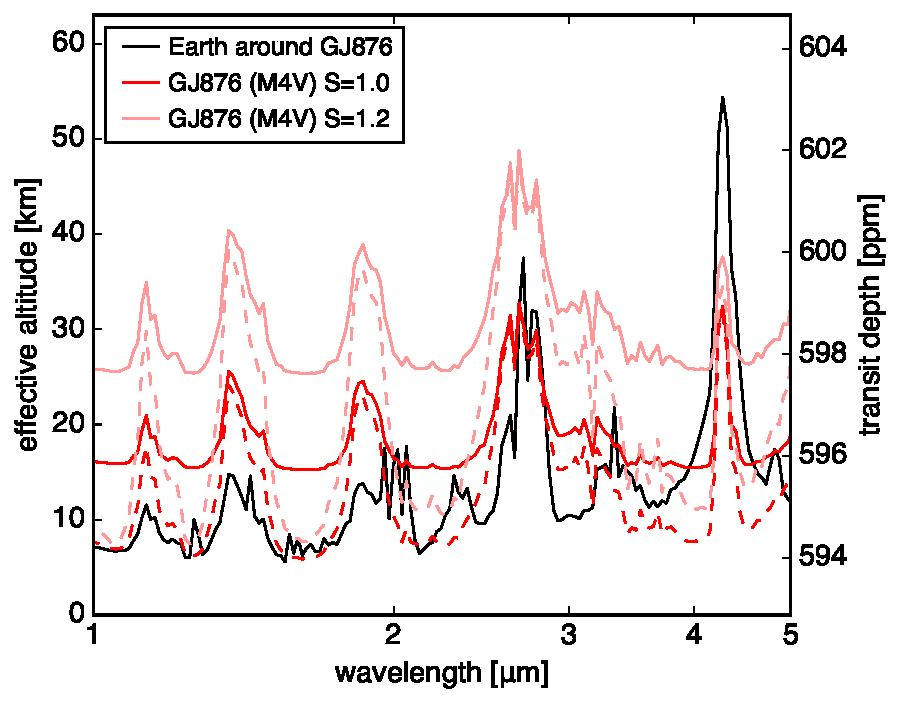
\includegraphics[width=\hsize]{fig/transit_GJ876.pdf}
    \end{center}
\caption{Red: Modeled transmission spectra based on GCM experiments for planets around GJ876 (M4V) with $S_X=0.6$ (dark red), $1.0$ (red) and $1.2$ (light red), with (solid) and without (dashed) clouds. The corresponding vertical profiles at the sub-stellar points are shown in Figure \ref{fig:AqOH0TLS_GJ876_temp_xH2O_vz_heat}. The left-hand side of the $y$-axis shows the effective altidue, while the right-hand side indicates the transit depth in ppm assuming the size of the star. }
\label{fig:transmission}
\end{figure}
%%%%%%%%%%%%%%%%%%%%%%%%%%%%%%%%%%%


%%%%%%%%%%%%%%%%%%%%%%%%%%%%%%%%%%%%%%%%%%%%%%%%%%%%%%%%%%%%%%%%%%%
\section{Sensitivity to varying parameters}
\label{s:sensitivity}
%%%%%%%%%%%%%%%%%%%%%%%%%%%%%%%%%%%%%%%%%%%%%%%%%%%%%%%%%%%%%%%%%%%

In this section, we examine the sensitivity of our results to the  assumptions we made. 
In particular, we consider the effect of spin rotation period (Section \ref{ss:sensitivity_Porbit}) and the effect of the assumption of the simple thermodynamic ocean, and then briefly discuss the effect of the background CO$_2$ mixing ratio. 


%%%%%%%%%%%%%%%%%%%%%%%%%%%%%%%%%%%%%%%%%%%%
\subsection{Effect of Orbital Period}
\label{ss:sensitivity_Porbit}
%%%%%%%%%%%%%%%%%%%%%%%%%%%%%%%%%%%%%%%%%%%%




In our fiducial set of experiments, we changed the orbital rotation period according to the Kepler's 3rd law to be consistent with the total incident flux the planet receives. 
Because we consider synchronously rotating planets, the spin rotation period has also been changed to match the orbital period. 
Thus, strictly speaking, the change in \water mixing ratio presented above includes both the effect of the varying incident flux ($S_X$) and the effect of varying rotation period. 
Although in Section \ref{s:results} we have discussed \water mixing ratio as a function of $S_X$, it is also known that the spin rotation period has non-negligible effects on the atmospheric circulation \citep{Yang2013, Kopparapu2016, Way2016} and thus would change \xwater. 
In this subsection, we check the effect of varying spin rotation period while fixing the total incident flux as well as keeping the assumption of synchronous rotation. 
% This admittedly leads to the configurations that do not realize, but tells us the degree of the effect of spin rotation period. 


%%%%%%%%%%%%%%%%%%%%%%%%%%%%%%%%%%%
\begin{figure}[!h]
    \begin{center}
    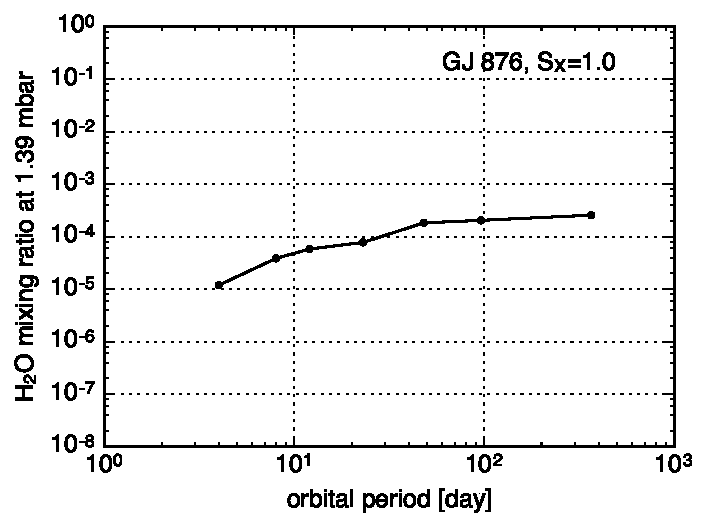
\includegraphics[width=\hsize]{fig/xH2O_Prot.pdf}
    \end{center}
\caption{The dependence of \water mixing ratio on the orbital(=spin) rotation period. }                                                                                                             
\label{fig:changeP}
\end{figure}
%%%%%%%%%%%%%%%%%%%%%%%%%%%%%%%%%%%

Figure \ref{fig:changeP} summarizes the results of the \water mixing ratio as a function of orbital(=spin) rotation period. 
The rotation period is changed from 4 Earth days to 1 Earth year. 
We find the trend where it increases as the rotation period decreases. 
This may also be explained by the 
\memo{Check the 3D profiles to explain this}. 



%%%%%%%%%%%%%%%%%%%%%%%%%%%%%%%%%%%%%%%%%%%%
\subsection{Effect of Ocean Model}
\label{ss:sensitivity_ocean}
%%%%%%%%%%%%%%%%%%%%%%%%%%%%%%%%%%%%%%%%%%%%


So far, we have used the thermodynamic ocean model with zero ocean heat transport and 50 m depth. 
Indeed, this simplified treatment has been regularly used in the published works of 3-dimensional atmospheric modeling for exoplanets. 
Yet, a more realistic approach is to include the dynamics of the ocean. 
Therefore, we check whether our results are sensitive to the prescription of ocean by comparing our fiducial results and those using a dynamic ocean module. 

For this purpose, we ran the models for GJ 876 assuming 900 m deep dynamic ocean. 
The models with the dynamic ocean typically equilibrated after a hundred to several hundreds of Earth years. 
In the same way as the fiducial models, we averaged the profile over approximately 10 Earth years after the model reached the steady state. 

Figure \ref{fig:change_ocean} shows \xwater for GJ876 with varying $S_X$ using the dynamic ocean module, in comparison with our fiducial results.  
There is a minor difference between the two, with the maximum difference being about the factor of 5 where the models with dynamic ocean tend to have lower \xwater. 
This is because \memo{I am not sure. This is just tentative. } with a dynamic ocean the heat absorbed by the surface is efficiently transported to the surrounding regions and the surface temperature at the sub-stellar point is lowered, weakening the convergence and convection there.
As the top altitude of convection is lowered, saturated \water mixing ratio becomes smaller because the atmospheric pressure is larger at lower atmosphere while the water pressure is fixed. 

Overall, however, our fiducial models with thermodynamic ocean approximation give a reasonable order-of-magnitude estimate for \water mixing ratio in the upper atmosphere. 

%%%%%%%%%%%%%%%%%%%%%%%%%%%%%%%%%%%
\begin{figure}[!h]
    \begin{center}
    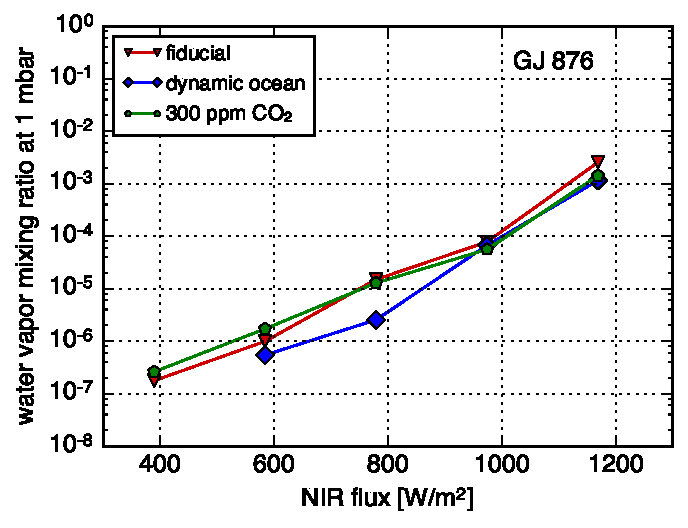
\includegraphics[width=0.9\hsize]{fig/xH2O_sensitivity.pdf}
    \end{center}
\caption{1.39 mbar \water mixing ratio of the models assuming dynamic ocean (blue diamond) and the models with Earth-like CO$_2$ mixing ratio (green pentagon), in comparison with the fiducial model with thermodynamic ocean and 1 ppm CO$_2$ (red down-triangle). }
\label{fig:change_ocean}
\end{figure}
%%%%%%%%%%%%%%%%%%%%%%%%%%%%%%%%%%%

%%%%%%%%%%%%%%%%%%%%%%%%%%%%%%%%%%%%%%%%%%%%
\subsection{Effect of CO$_2$}
\label{ss:sensitivity_ocean}
%%%%%%%%%%%%%%%%%%%%%%%%%%%%%%%%%%%%%%%%%%%%

Our fiducial models assumed 1 ppm CO$_2$, which was an arbitrary choice. 
Although a full investigation of the dependence on the CO$_2$ mixing ratio is beyond the scope of this paper, here we briefly mention how much the results are changed if we assume an Earth-like CO$_2$ mixing ratio. 
The results of the models with 300 ppm of CO$_2$ are plotted in Figure \ref{fig:change_ocean}. 
As shown, this level of variation of CO$_2$ has a very small effect on the \water profile. 
Larger amounts of CO$_2$ up to that for CO$_2$-dominated atmosphere could have a more substantial effect on the 3D profiles \citep{Wordsworth2013}. 


%%%%%%%%%%%%%%%%%%%%%%%%%%%%%%%%%%%%%%%%%%%%%%%%%%%%%%%%%%%%%%%%%%%
\section{Summary and Discussion}
\label{s:summary}
%%%%%%%%%%%%%%%%%%%%%%%%%%%%%%%%%%%%%%%%%%%%%%%%%%%%%%%%%%%%%%%%%%%

We have investigated the response of \water profiles of synchronously rotating planets to the change in the incident stellar flux. 
We find a gradual (quasi-exponential) increase of \water mixing ratio in the upper atmosphere as a function of incident flux, resulting in the several orders of magnitude variation as total incident flux increases by a factor of 2-3. 

Due to the stabilized surface temperature at the sub-stellar point, the increase of \water mixing ratio in response to larger incident flux is not primarily caused by the increased surface temperature as previous 1D models suggest. 
Instead, it is induced by the increased near-infrared portion of the incident flux. 
The enhanced radiative heating due to the absorption by \water drives upward motion of the air, which takes over the role of transporting \water mixing ratio from the moist lower atmosphere to the upper atmosphere, further increasing the heating rate in the upper atmosphere.
As a result, the moisture in the upper atmosphere increases dramatically while the surface temperature below it remains temperate. 
This picture is supported by the good correlation between the \water mixing ratio at \preslevel and the near-infrared portion of the incident radiation, regardless of the spectral type of the host star. 

Simulating transmission spectra based on the atmospheric profiles found by GCM experiments, 
we demonstrate that the increase \preslevel \water mixing ratio from $10^{-6}$ to $3 \times 10^{-3}$ corresponds to the increase of the \water absorption depth by a factor of a few, making the effective altitude of \water as high as 40~km. 
The presence of clouds in the high atmosphere on the terminator potentially increases the baseline effective altitude and thus weakens the absorption features. 
We bracketed the effect of clouds in the transmission spectra, 
although there are uncertainties in the detailed optical properties of cloud particles as well as in the cloud formation processes in any GCM treatment. 

While we used a thermodynamic ocean model with zero ocean heat transport for simplicity, comparable experiments with a dynamic ocean are also performed to demonstrate that this approximation of ocean results is a minor effect on the \water mixing ratio within an order of magnitude. 
We also confirmed that the effect of the change in the planet spin period has a secondary effect, resulting in an order of magnitude variation at most. 
Varying CO$_2$ level from 1~ppm to 300~ppm has only a negligible effect. 

In this paper, we limit our discussion on the \water profiles to the effects of the total incident flux and spectral energy distribution (i.e., the spectral types of the host star). 
These parameters are among the limited number of properties that can be constrained relatively easily from the observations of exoplanets. 
In principle, however, \water distributions also depend on geophysical parameters including the surface gravity and atmospheric pressure, as well as photochemistry that depends on detailed atmospheric composition. 
These could perhaps be constrained by retrievals from observed planetary spectra to give a prediction for \water mixing ratio in the upper atmosphere, but  otherwise could rather be inferred from the \water mixing ratio. 
The dependence on these planetary properties will be a focus of future study. 





\acknowledgments
We thank Micheal J. Way and Nancy Y. Kiang for providing the boundary conditions for \modelE \ and for the helpful discussions. 
The support from Maxwell Kelley and Igor Aleinov was critical in resolving the issues identified in the process of generalizing \modelE for exotic configurations considered in this paper. 
Y.~F. is deeply grateful to David S. Spiegel for the insightful discussions on the simulation suite for transmission spectra. 
Y.~F. also acknowledges the generous support from Universities Space Research Association (USRA) through the NASA Postdoctoral Program. 
We appreciate the supported by the NASA's NExSS project. 

\bibliography{GCM_qstrato_ref}


\appendix


%%%%%%%%%%%%%%%%%%%%%%%%%%%%%%%%%%%%%%%%%%%%%%%%%%%%%%%%%%%%%%%%%%%
\section{Validation of radiation scheme used in our GCM}
\label{ap:radiation}
%%%%%%%%%%%%%%%%%%%%%%%%%%%%%%%%%%%%%%%%%%%%%%%%%%%%%%%%%%%%%%%%%%%

In this paper, we applied a GCM named ROCKE-3D to planets around the stars with different spectral types. 
In doing so, a special caution needed to be taken regarding the accuracy of the radiative transfer calculation, because the baseline model of ROCKE-3D has been developed for the Earth, and the radiative transfer calculation was optimized for solar insolation. 
We therefore implemented the SOCRATES radiation scheme, which is easier to generalize to different planetary conditions.

In order to check the accuracy of the radiative transfer calculation used in the GCM, we compare it with a more accurate high-spectral-resolution calculation assuming the same (1-dimensional) atmospheric profile. 
The atmospheric profile to test was the one at the sub-stellar point of a planet around GJ876 with $S_X=1.2$ (see Figure \ref{fig:AqOH0TLS_GJ876_temp_xH2O_vz_heat}), but without clouds. 
This profile was chosen because of its extremely high \water mixing ratio, which is very different from the Earth. 
Assuming that profile, we calculated short wave radiative transfer with 29 bands (used in the GCM) and with 280 bands, both for the cases of solar incident flux and the incident flux of GJ876. 

We show in Figure \ref{fig:socrates} the short-wave (stellar) downward flux, upward flux and heating rate obtained both with the 29 bands used in the GCM and with a benchmark set-up with 280 bands. Differences are small, $<$ 5 W/m$^2$ for fluxes and $<$ 0.5 K/day for the heating rate except at pressures $\ll$ 1 mbar, throughout the atmosphere. We therefore conclude that the radiation scheme adopted here is sufficiently accurate.

%%%%%%%%%%%%%%%%%%%%%%%%%%%%%%%%%%%
\begin{figure*}[!htb]
    \begin{center}
    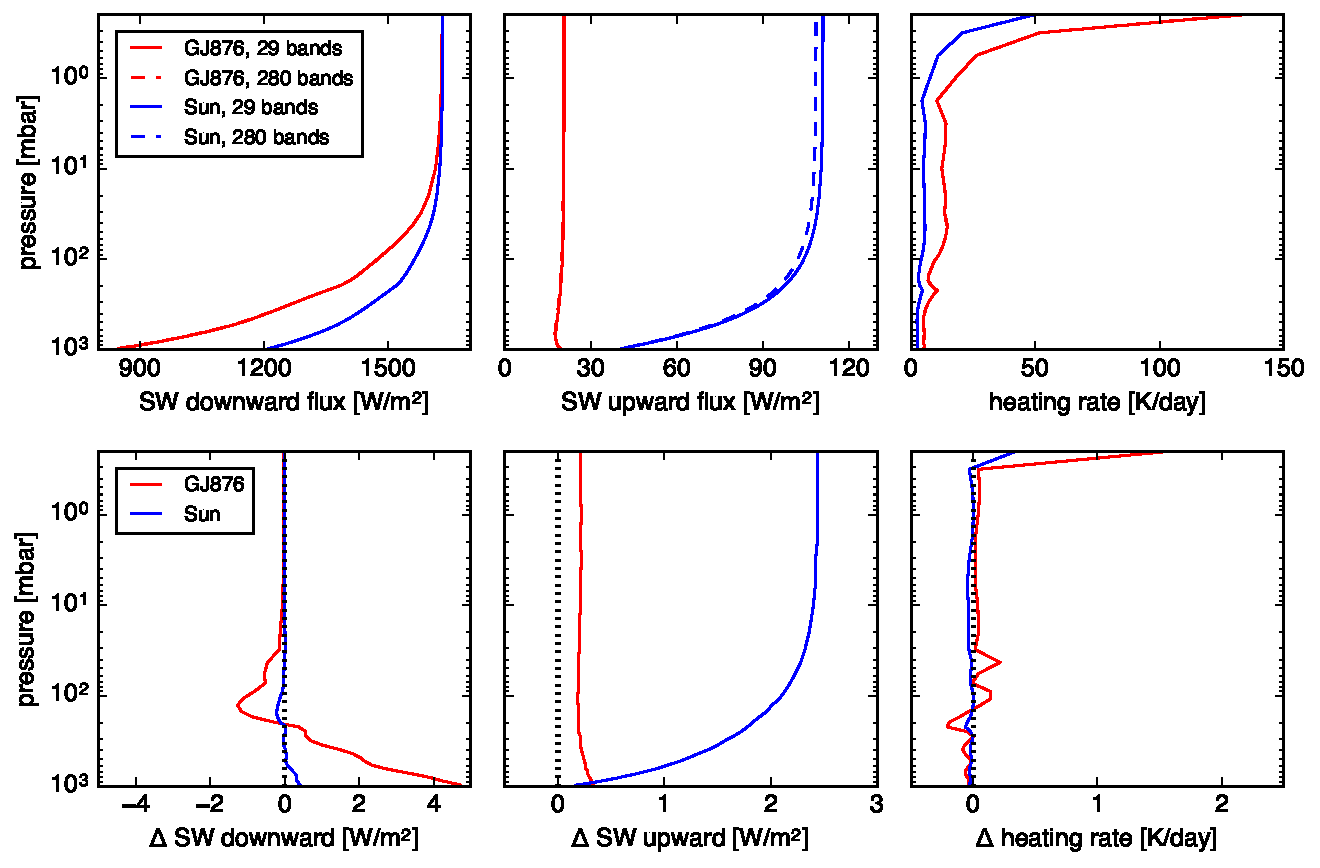
\includegraphics[width=0.8\hsize]{fig/rad_comparison_SW29-SW280_AqOH0TLS_GJ876S12P20L40Q.pdf}
    \end{center}
\caption{Comparison in shortwave downward flux (left), upward flux (center), and the heating rate (left) between 29-band models used in GCM and 280-band models. The atmospheric profile assumed is the one at the substellar point of a planet around GJ 876 with $S_X=1.2$ (see the upper panels of Figure \ref{fig:AqOH0TLS_GJ876_temp_xH2O_vz_heat}). }
\label{fig:socrates}
\end{figure*}
%%%%%%%%%%%%%%%%%%%%%%%%%%%%%%%%%%%



\begin{table}
\centering
\caption{The short-wave bands.}
\label{tab:short-wave}
\begin{tabular}{l|l|l} \hline \hline
\# & lower limit [${\rm m}$m] & upper limit [${\rm m}$m] \\ \hline 
    1 &       0.200 &    0.385 \\
    2 &       0.385 &    0.500 \\
    3 &       0.500 &    0.690 \\
    4 &       0.690 &    0.870 \\
    5 &       0.870 &    0.900 \\
    6 &       0.900 &    1.08 \\
    7 &       1.08  &   1.12 \\
    8 &       1.12  &   1.16 \\
    9 &       1.16  &   1.20 \\
   10 &       1.20  &   1.30 \\
   11 &       1.30  &   1.34 \\
   12 &       1.34  &   1.42 \\
   13 &       1.42  &   1.46 \\
   14 &       1.46  &   1.52 \\
   15 &       1.52  &   1.56 \\
   16 &       1.56  &   1.62 \\
   17 &       1.62  &   1.68 \\
   18 &       1.68  &   1.80 \\
   19 &       1.80  &   1.94 \\
   20 &       1.94  &   2.00 \\
   21 &       2.00  &   2.14 \\
   22 &       2.14  &   2.50 \\
   23 &       2.50  &   2.65 \\
   24 &       2.65  &   2.85 \\
   25 &       2.85  &   3.15 \\
   26 &       3.15  &   3.60 \\
   27 &       3.60  &   4.10 \\
   28 &       4.10  &   4.60 \\
   29 &       4.60  &   10.0 \\ \hline
\end{tabular}
\end{table}



%%%%%%%%%%%%%%%%%%%%%%%%%%%%%%%%%%%
%\begin{figure*}[!htb]
%    \begin{center}
%    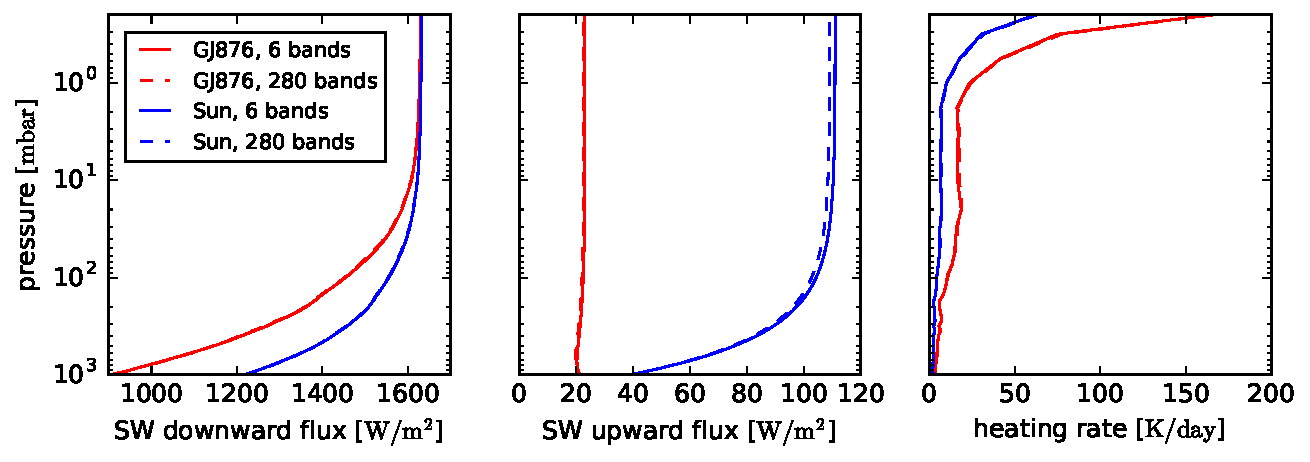
\includegraphics[width=0.8\hsize]{rad_comparison_AqOH0TLS_GJ876S12P21L40Q.eps}
%    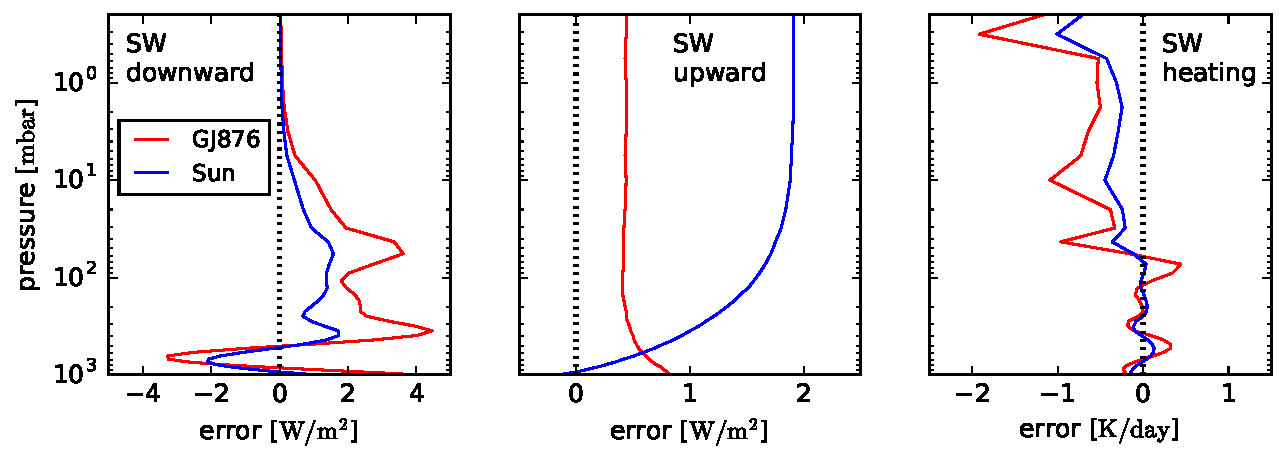
\includegraphics[width=0.8\hsize]{rad_comparison_diff_AqOH0TLS_GJ876S12P21L40Q.pdf}
%    \end{center}
%\caption{}                                                                                                             
%\label{fig:}
%\end{figure*}
%%%%%%%%%%%%%%%%%%%%%%%%%%%%%%%%%%%



\end{document}


